\documentclass[a4paper,11pt]{article}
\usepackage{dmasproject}
% if you need additional LaTeX packages, add them here

\title{Your Project Title Goes Here}
% sort your names alphabetically by last name
\author{
  First Author (s123456)
  \\
  Second Author (s234567)
  \\
  Third Author (s345678)
  \\
  Fourth Author (s456789)
}
\date{Alpha version, September 2020} % change this accordingly

\begin{document}

\maketitle

\begin{abstract}
The abstract should briefly summarize your project in 150--250 words.
\end{abstract}

\section{Introduction}

You can also refer to more general literature here, for example~\cite{WooldridgeMAS} or~\cite{wiki:SchellingSegregation}.

\subsection{Problem}

Key question 1: What is the problem addressed?

\subsection{State of the art}

Key question 2: What is the state of the art concerning this problem?
Which publications are the inspiration for your project?
Add them to the file \texttt{references.bib} and cite them like this~\cite{dWVV2013:ToM}.

Note that the \verb|\cite| command can take multiple references~\cite{vDGKK2019:ReachGossip,vdBerg2019:UnreliableGossip,HvKLL2019:SupermarketQ}.

\subsection{New idea}

Key question 3: What is the new idea for addressing the problem?

\section{Method}

\subsection{Simulation model}

Here you should describe your model.
How similar to the one used in your state of the art reference is it?
Which things did you change, and why?

\begin{figure}[h]
  \centering
  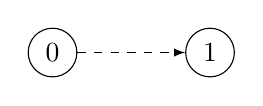
\begin{tikzpicture}[node distance=2cm,>=latex]
    \node (0) [circle,draw] {0};
    \node (1) [circle,draw,right of=0] {1};
    \draw [->,dashed] (0) -- (1);
  \end{tikzpicture}
  \caption{A figure should always have a caption.}\label{fig1:twoDots}
\end{figure}

If you add figures, such as \autoref{fig1:twoDots}, always refer to them at least once.
Please use tikz or vector formats like EPS or PDF.
Avoid pixel formats such as PNG or JPG (because they would become pixelated or blurry).

\subsection{Implementation details}

Here you should describe the implementation of your simulation.
Please explicitly mention any programming languages, tools or libraries you used.

\subsection{Experiment design}

Did you run multiple different versions of your simulation with different parameters?
Then explain the different setups here and why you chose them.

You can also mention here what results you are expecting.

\section{Results}

\subsection{Experiment findings}

Key question 4: What are the results you obtained?

It can be good to use a Table, like \autoref{tab1:results}.
Please ensure that numeric results are right-aligned and have the same number of digits, to allow for easy comparison.

\begin{table}[h]
  \centering
  \begin{tabular}{lrr}
    \toprule
    Setup & run time & success rate \\
    \midrule
    1  & 0.123 & 12\% \\
    2  & 0.456 & 34\% \\
    3a & 0.789 & 56\% \\
    3b & 1.234 & 78\% \\
    \bottomrule
  \end{tabular}
  \caption{Tables should always have a caption.}\label{tab1:results}
\end{table}

You might also want to include plots or graphs.
Similar to figures, please do not use screenshots or pixel-based formats, but vector-based formats.
Alternatively, generate your plots with the \texttt{pgfplots} package as done here in Figure~\ref{fig1:plot}.

\begin{figure}[h]
  \centering
  \begin{tikzpicture}
    % ideally the results.txt file should be automatically generated by your implementation.
    \pgfplotstableread{results.txt}\datatable
    \begin{axis}
      \addplot+[error bars/.cd, y dir=both, y explicit, error bar style={color=black}] table[x=day, y=explosions, y error=explosionsSD] from \datatable;
      \addplot+[error bars/.cd, y dir=both, y explicit, error bar style={color=black}] table[x=day, y=fires, y error=firesSD] from \datatable;
      \legend{explosions, fires};
    \end{axis}
  \end{tikzpicture}
  \caption{Figures should also have a caption.}\label{fig1:plot}
\end{figure}

\subsection{Interpretation of findings}

Summarise your results.
Are the results what you expected?
Which results are surprising?
How do you interpret them?

\section{Conclusion}
\subsection{Discussion}

What do you take away from your project?
What did you learn?

\subsection{Relevance}

Key question 5: What is the relevance of this work?

Which new questions do you have now?
Do you results suggest future research directions?

\subsection{Team Work}

How did you work together as a team?
Who contributed how to this report and to the implementation?
What should you have done differently?

% This will print you references, please do not change it.
\printbibliography

\end{document}
